\documentclass[10pt,a4paper]{article}
\usepackage{tocloft}
\usepackage{commons/course}
\usepackage{booktabs}
\usepackage{graphicx}
\usepackage{tikz}
\usetikzlibrary{arrows.meta,positioning,calc,decorations.pathreplacing}

\definecolor{keywordstyle}{rgb}{0.0, 0.4, 0.8}
\definecolor{stringstyle}{rgb}{0.9, 0.17, 0.31}
\definecolor{commentstyle}{rgb}{0.1, 0.6, 0.2}
\definecolor{numberstyle}{rgb}{0.4, 0.4, 0.4}
\definecolor{backgroundcolor}{rgb}{0.94, 0.97, 1.0}

\lstdefinelanguage{ShellLike}{
	morekeywords={PASS,FAIL,Passed,Failed,Running,Loading,summary,iverilog},
	sensitive=false,
	morecomment=[l]{\#},
	morestring=[b]",
}

\lstset{
	language=ShellLike,
	basicstyle=\ttfamily\scriptsize,
	keywordstyle=\color{keywordstyle}\bfseries,
	stringstyle=\color{stringstyle},
	commentstyle=\color{commentstyle},
	numbers=none,
	keepspaces=true,
	tabsize=2,
	showspaces=false,
	showstringspaces=false,
	showtabs=false,
	breaklines=true,
	breakatwhitespace=false,
	frame=single,
	backgroundcolor=\color{backgroundcolor},
}

\lstdefinestyle{verilog}{
	language=Verilog,
	basicstyle=\ttfamily\scriptsize,
	keywordstyle=\color{keywordstyle}\bfseries,
	commentstyle=\color{commentstyle},
	stringstyle=\color{stringstyle},
	numbers=left,
	numberstyle=\tiny\color{numberstyle},
	frame=single,
	backgroundcolor=\color{backgroundcolor},
	breaklines=true,
	tabsize=2,
}

\newlistof{listofproblems}{lop}{\normalsize فهرست مسائل}
\newcommand{\addproblem}[1]{\addcontentsline{lop}{listofproblems}{\protect\numberline{}#1}}

\begin{document}

\سربرگ{آزمایش چهارم}{توصیف رفتاری (پشته‌ی \lr{LIFO})}{}{استاد: دکتر انصاری}

\subsubsection*{خلاصه}

در این آزمایش یک پشته‌ی \lr{LIFO} با عمق ۸ کلمه و پهنای ۴ بیت با توصیف {رفتاری} (\lr{behavioral}) در \lr{Verilog} پیاده‌سازی شده است. برخلاف آزمایش قبل که همه‌چیز با \lr{assign} نوشته می‌شد، اینجا کل ماژول با بلوک‌های \lr{always} توصیف می‌شود: یک بلوک ترتیبی همگام با لبه‌ی بالارونده‌ی کلاک برای حافظه و اشاره‌گر پشته، و یک بلوک ترکیبی \lr{always @(*)} برای خروجی داده.

صحت‌سنجی با \lr{Icarus Verilog} (\lr{iverilog}/\lr{vvp}) و به کمک یک {مدل مرجع} مستقل انجام شده است؛ مدل مرجع در تست‌بنچ به‌صورت جداگانه پیاده شده و خروجی طراحی در هر لبه‌ی کلاک با آن مقایسه می‌شود.

\subsubsection*{مشخصات واسط}

ورودی‌ها و خروجی‌های خواسته‌شده در صورت آزمایش به این شکل پیاده شده‌اند:

\begin{center}
\begin{tabular}{@{}lll p{7.2cm}@{}}
\toprule
{سیگنال} & {جهت} & {پهنا} & {توضیح} \\
\midrule
\lr{Clk}      & ورودی & ۱ & کلاک؛ همه‌ی تغییرات حالت روی لبه‌ی بالارونده \\
\lr{RstN}     & ورودی & ۱ & ریست ناهم‌گام فعال‌پایین؛ پشته را خالی می‌کند \\
\lr{Data\_In} & ورودی & ۴ & داده‌ی ورودی برای \lr{Push} \\
\lr{Push}     & ورودی & ۱ & فرمان نوشتن روی سر پشته \\
\lr{Pop}      & ورودی & ۱ & فرمان برداشتن از سر پشته \\
\lr{Data\_Out}& خروجی & ۴ & کلمه‌ی روی سر پشته (خواندن ترکیبی) \\
\lr{Full}     & خروجی & ۱ & $\mathrm{Full}=1$ یعنی پشته پر است \\
\lr{Empty}    & خروجی & ۱ & $\mathrm{Empty}=1$ یعنی پشته خالی است \\
\bottomrule
\end{tabular}
\end{center}

نام سیگنال ریست در صورت آزمایش \lr{RstN} است؛ پسوند \lr{N} قرارداد رایج برای {فعال‌پایین} بودن است، بنابراین ریست به‌صورت ناهم‌گام و فعال‌پایین (\lr{negedge RstN}) پیاده شده است.

 در صورت آزمایش نوشته شده \lr{Empty=0 indicates that the stack is empty} که با سطر بالایی آن (\lr{Full=1 indicates that the stack is full}) ناسازگار است؛ اگر $\mathrm{Empty}=0$ به معنی خالی بودن باشد، آنگاه پرچم عملا یک سیگنال \lr{Not-Empty} است و نامش گمراه‌کننده می‌شود. در این پیاده‌سازی قرارداد متعارف و متقارن با \lr{Full} انتخاب شده است، یعنی $\mathrm{Empty}=1$ به معنی خالی بودن پشته. اگر مقصود صورت آزمایش دقیقا همان متن باشد، تنها کافی است خروجی معکوس شود:

\begin{latin}
\begin{lstlisting}[style=verilog,numbers=none]
assign Empty = ~(sp == 0);
\end{lstlisting}
\end{latin}

\subsubsection*{ساختار داخلی}

پشته با یک آرایه‌ی حافظه و یک اشاره‌گر توصیف می‌شود. اشاره‌گر \lr{sp} برابر {تعداد کلمات معتبر} داخل پشته است، نه اندیس خانه‌ی بالایی؛ این انتخاب باعث می‌شود پرچم‌ها بسیار ساده شوند:

\[
\begin{aligned}
\mathrm{Empty} &= (\mathrm{sp} = 0)\\
\mathrm{Full}  &= (\mathrm{sp} = \mathrm{DEPTH})\\
\mathrm{Data\_Out} &= \begin{cases} 0 & \mathrm{sp} = 0\\ \mathrm{mem}[\mathrm{sp}-1] & \text{در غیر این صورت}\end{cases}
\end{aligned}
\]

چون \lr{sp} باید بتواند هر دو مقدار $0$ و $\mathrm{DEPTH}$ را نگه دارد، پهنای آن $\lceil \log_2 \mathrm{DEPTH}\rceil + 1$ بیت است (برای عمق ۸ یعنی ۴ بیت). اگر اشتباها ۳ بیت گرفته می‌شد، مقدار ۸ به ۰ سرریز می‌کرد و پشته‌ی پر با پشته‌ی خالی اشتباه گرفته می‌شد.

\begin{center}
\begin{latin}
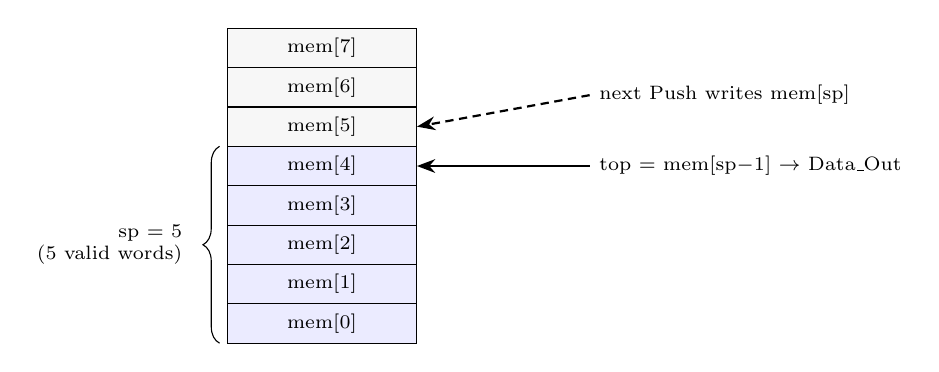
\begin{tikzpicture}[
  cell/.style={draw, minimum width=2.4cm, minimum height=0.5cm, align=center, font=\scriptsize},
  used/.style={cell, fill=blue!8},
  free/.style={cell, fill=black!3},
  >=Stealth
]
  \node[free] (m7) at (0,3.5)  {mem[7]};
  \node[free] (m6) at (0,3.0)  {mem[6]};
  \node[free] (m5) at (0,2.5)  {mem[5]};
  \node[used] (m4) at (0,2.0)  {mem[4]};
  \node[used] (m3) at (0,1.5)  {mem[3]};
  \node[used] (m2) at (0,1.0)  {mem[2]};
  \node[used] (m1) at (0,0.5)  {mem[1]};
  \node[used] (m0) at (0,0.0)  {mem[0]};

  % top-of-stack pointer
  \node[font=\scriptsize, anchor=west] (toplbl) at (3.4,2.0)
      {top $=$ mem[sp$-$1] $\rightarrow$ Data\_Out};
  \draw[->, thick] (toplbl.west) -- (m4.east);

  % next push slot
  \node[font=\scriptsize, anchor=west] (nxtlbl) at (3.4,2.9)
      {next Push writes mem[sp]};
  \draw[->, thick, densely dashed] (nxtlbl.west) -- (m5.east);

  % occupancy brace
  \draw[decorate, decoration={brace, amplitude=6pt}] (-1.3,-0.25) -- (-1.3,2.25);
  \node[font=\scriptsize, align=right, anchor=east] at (-1.65,1.0)
      {sp $=$ 5\\(5 valid words)};
\end{tikzpicture}
\end{latin}
\end{center}

\subsubsection*{داوری فرمان‌ها}

چهار حالت مرزی وجود دارد که باید صریحا مشخص شوند، وگرنه مدار در شرایط لبه‌ای رفتار نامعین پیدا می‌کند:

\begin{center}
\begin{tabular}{@{}ll p{8.2cm}@{}}
\toprule
{وضعیت} & {رفتار} & {دلیل} \\
\midrule
\lr{Push} و پشته پر    & نادیده گرفته می‌شود & جلوگیری از \lr{overflow}؛ داده‌ی قدیمی خراب نمی‌شود \\
\lr{Pop} و پشته خالی   & نادیده گرفته می‌شود & جلوگیری از \lr{underflow}؛ \lr{sp} منفی نمی‌شود \\
\lr{Push} و \lr{Pop} همزمان & هیچ کاری انجام نمی‌شود & دو فرمان مستقل و متناقض؛ امن‌ترین تفسیر \\
هیچ‌کدام فعال نیست     & حالت حفظ می‌شود & \\
\bottomrule
\end{tabular}
\end{center}

این داوری در دو سیگنال کمکی خلاصه شده است تا بدنه‌ی بلوک \lr{always} تمیز بماند:

\begin{latin}
\begin{lstlisting}[style=verilog,numbers=none]
wire do_push = Push & ~Pop & ~Full;
wire do_pop  = Pop  & ~Push & ~Empty;
\end{lstlisting}
\end{latin}

توجه کنید که برای \lr{Push} و \lr{Pop} همزمان می‌شد رفتار \lr{replace top} (جایگزینی سر پشته) را هم انتخاب کرد؛ اما صورت آزمایش این دو را دو فرمان مستقل تعریف کرده و چیزی درباره‌ی ترکیبشان نگفته است، پس تفسیر محافظه‌کارانه‌ی بدون تغییر انتخاب شده و در تست‌بنچ هم صریحا آزموده می‌شود.

\pagebreak


\subsubsection*{کد طراحی}

ماژول کاملا رفتاری است: حافظه و اشاره‌گر در یک \lr{always @(posedge Clk or negedge RstN)} و خروجی داده در یک \lr{always @(*)} توصیف شده‌اند. پارامترهای \lr{WIDTH} و \lr{DEPTH} پیش‌فرض همان مقادیر خواسته‌شده در صورت آزمایش هستند.


\begin{latin}
\lstinputlisting[style=verilog]{../rtl/stack.v}
\end{latin}

\pagebreak


\subsubsection*{شکل موج}

سناریوی شکل‌موج طوری چیده شده که همه‌ی رفتارهای مرزی در یک تصویر دیده شوند: ابتدا ریست ناهم‌گام (پشته خالی و $\mathrm{Empty}=1$)، سپس یک \lr{Pop} روی پشته‌ی خالی که نادیده گرفته می‌شود، سپس هشت \lr{Push} پیاپی با مقادیر $1$ تا $8$، سپس یک \lr{Push} با مقدار $\mathrm{F}$ روی پشته‌ی پر که نباید اثری بگذارد، و در پایان هشت \lr{Pop} که داده‌ها را دقیقا به ترتیب معکوس بازمی‌گردانند.

\begin{center}
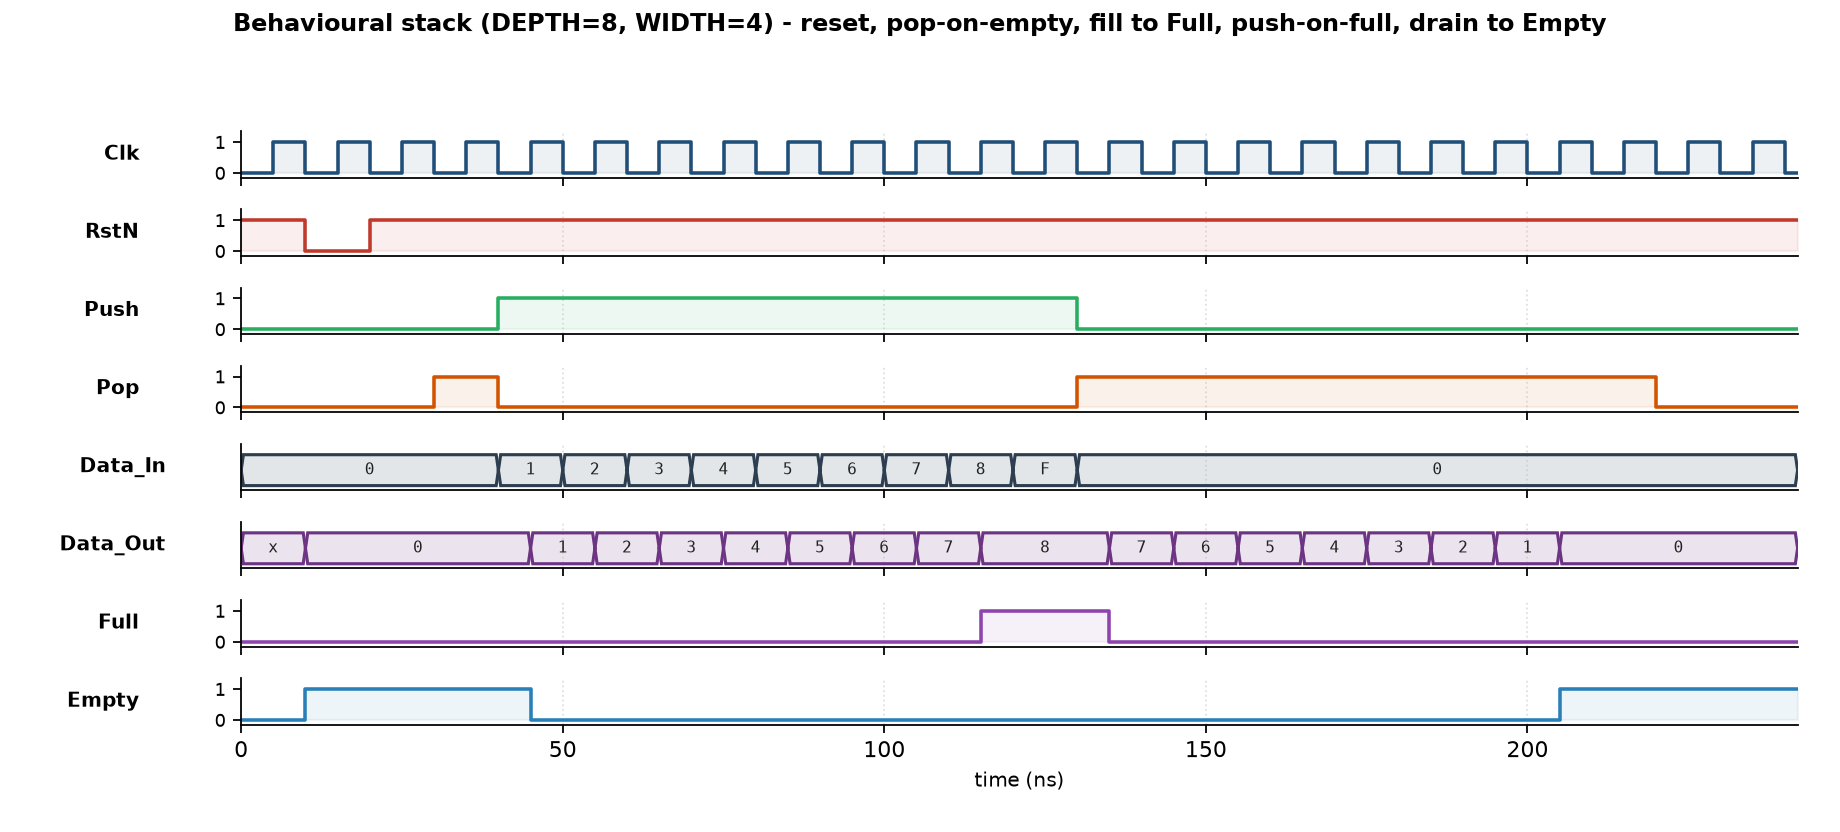
\includegraphics[width=\textwidth]{figs/wave_stack.png}\\[0.4em]
\end{center}

چند نکته در شکل بالا قابل مشاهده است. پرچم \lr{Full} دقیقا روی هشتمین \lr{Push} بالا می‌رود و نه زودتر؛ در بازه‌ای که \lr{Full} فعال است و \lr{Data\_In} برابر $\mathrm{F}$ می‌شود، مقدار \lr{Data\_Out} روی $8$ ثابت می‌ماند که یعنی سرریز واقعا بلوکه شده است. در بخش تخلیه، \lr{Data\_Out} دنباله‌ی $8,7,6,\dots,1$ را طی می‌کند که همان ترتیب \lr{LIFO} است، و در انتها \lr{Empty} دوباره فعال شده و \lr{Data\_Out} به $0$ برمی‌گردد.

\pagebreak

\subsubsection*{تست‌بنچ اصلی}

تست‌بنچ به جای مقایسه با مقادیر ثابت دستی، یک {مدل مرجع} مستقل نگه می‌دارد (آرایه‌ی \lr{ref\_mem} و شمارنده‌ی \lr{ref\_sp}) و بعد از هر لبه‌ی کلاک، هر سه خروجی \lr{Data\_Out}، \lr{Full} و \lr{Empty} را با مدل مقایسه می‌کند. تحریک ورودی‌ها روی لبه‌ی پایین‌رونده اعمال می‌شود تا شرایط \lr{setup/hold} حول لبه‌ی بالارونده هیچ‌وقت مبهم نباشد.

سناریوهای پوشش‌داده‌شده به ترتیب عبارت‌اند از: ریست ناهم‌گام، \lr{Pop} روی پشته‌ی خالی، پرکردن کامل تا \lr{Full}، \lr{Push} روی پشته‌ی پر، تخلیه‌ی کامل و بررسی ترتیب \lr{LIFO}، سیکل‌های بیکار، \lr{Push} و \lr{Pop} همزمان در سه عمق مختلف (خالی، میانه، پر)، ریست از حالت غیرخالی، الگوی درهم‌آمیخته‌ی \lr{push/pop}، و در پایان ۲۰۰۰ فرمان {تصادفی} که مستقیما با مدل مرجع مقایسه می‌شوند.

\begin{latin}
\lstinputlisting[style=verilog]{../tb/tb_stack.v}
\end{latin}

\pagebreak

\subsubsection*{تست‌بنچ پارامتری}

علاوه بر تست اصلی، یک تست‌بنچ دوم همان ماژول را با سه هندسه‌ی متفاوت می‌سازد: $(\mathrm{WIDTH},\mathrm{DEPTH})$ برابر $(4,8)$ یعنی همان چیزی که صورت آزمایش خواسته، و همچنین $(8,4)$ و $(2,16)$. هدف این است که مطمئن شویم عمق و پهنا واقعا پارامتری‌اند و جایی در کد به‌صورت ثابت فرض نشده‌اند؛ به‌ویژه محاسبه‌ی پهنای اشاره‌گر که در صورت اشتباه، دقیقا در حالت \lr{Full} خودش را نشان می‌دهد.

\begin{latin}
\lstinputlisting[style=verilog]{../tb/tb_stack_param.v}
\end{latin}

\subsubsection*{نتایج تست}


\begin{latin}
\lstinputlisting[basicstyle=\ttfamily\scriptsize]{figs/test_run_output.txt}
\end{latin}

\pagebreak

\subsubsection*{جمع‌بندی}

تفاوت اصلی این آزمایش با آزمایش قبل در {سطح توصیف} است. در توصیف جریان داده باید خود معادلات منطقی نوشته می‌شد، اما در توصیف رفتاری کافی است {رفتار} مدار را بیان کنیم و ساخت حافظه، شمارنده و منطق کنترلی به ابزار سنتز سپرده شود. همین باعث می‌شود پیاده‌سازی پشته‌ای که در سطح گیت کار نسبتا سنگینی است، در چند خط \lr{always} خلاصه شود.

نکته‌ی مهم دیگر این است که در توصیف رفتاری، حالت‌های مرزی به‌طور خودکار امن نمی‌شوند؛ سرریز، تهی‌خوانی و فرمان‌های متناقض باید صریحا در کد مدیریت شوند، وگرنه اشاره‌گر پشته می‌تواند از محدوده خارج شود. به همین دلیل بخش عمده‌ی تست‌بنچ به همین حالت‌ها اختصاص یافته است.

\end{document}
